\documentclass[12pt]{article}
\usepackage[utf8]{inputenc}
\usepackage{amsmath}
\usepackage{graphicx}
\usepackage{listings}
\usepackage{enumitem}
\usepackage{tcolorbox}
\usepackage{braket}

\title{Computational Complexity Assignment 2}

\author{Tyler Tracy}

\newtcolorbox{questionbox}{
        colframe=cyan!20!white,
        colback =cyan!20!white,
        top=0mm, bottom=0mm, left=0mm, right=0mm,
        arc=0mm,
%
        fontupper=\color{blue!70!black},
        fonttitle=\bfseries\color{blue!70!black},
        title=Question:
                        }

\setlength{\parskip}{\baselineskip}%
\setlength{\parindent}{0pt}%

\begin{document}

\maketitle


\section*{Problem 1}

\begin{questionbox}
	A tree is a connected graph which contains no cycles. Let $TREE = \{ \braket{G} \mid G \text{ is a tree } \}$. Prove that $TREE \in P$.
\end{questionbox}

To prove that a problem is a member of $P$, we must find an algorithm that can decide the problem in polynomial time.

To solve this problem, I'll use a version of depth first search. The algorithm will loop over all nodes and start traversing each node, if any encountered node has already been visited and is not the parent of the current node, then we know that there is a cycle in the graph. The algorithm loops over all possible nodes doing this in case there are multiple disconnected components in the graph.

Below I give a pseudocode implementation of the above algorithm and analyze its running time.

\begin{lstlisting}[basicstyle=\small, tabsize=3]
	fn ContainsCycle(G: Graph) -> bool:
		visited = []
		fn ContainsCycleInner(G: Graph, v: int) -> bool:
			visited[v] = true
			for each w in G.adjacentNodes(v):
				hasVisited = visited[w]
				isParent = G.adjacentNode(w).contains(v)
				if isParent
					continue
				if hasVisited:
					return true
				return ContainsCycleInner(G, w)
			return false

		for each w in G.nodes():
			if visited[w]:
				continue
			if ContainsCycleInner(G, w):
				return true
		return false
\end{lstlisting}

It isn't explicit in the loop, but the loop will visit each node at most once. This is because the loop will only visit a node if it has not been visited yet. It will also only visit each edge once because each edge can only be reached from a single node and each node is only visited once. It is useful to refer to the size of these sets so I will set $N = |V| + |E|$

I'll assume that the computational model allows for dictionary lookups and writes in $O(ln(n))$ time. Where $n$ is the size of the key and $ln(n)$ represents the number of bits needed to store $n$. The idea behind this assumption is the need to read the digits of the object and perform some computation on them. If the graph structure is well encoded, looking up a node or adjacent nodes will take $O(ln(n))$.

So for each node, we potentially have to loop over its adjacent nodes and write to a dictionary. This means that the time complexity of the algorithm is $O(Nln(N))$. Since this complexity is polynomial in the size of the input, this algorithm is a member of $P$. Thus $TREE \in P$

\section*{Problem 2}

\begin{questionbox}
	Given a graph $G$, a coloring of $G$ with $c$ colors is an assignment of a number in $[c]$ (i.e 0 through $c-1$) to each vertex such that no adjacent vertices get the same number. Let $2COL = \{ \braket{G, c} \mid G \text{ is a graph which has a coloring with 2 colors} \}$. Prove that $2COL \in NP$.
\end{questionbox}

To prove that a problem is a member of $NP$, we must find a polynomial time algorithm that given the input an a certificate, can verify that the certificate is a valid solution to the problem.

The certificate for $2COL$ is the actual coloring of the graph. This can be represented as some mappings of each node to some number $c$.

The basic idea of an algorithm to solve this problem is to read the coloring of the graph and check each node to see if it is connected to any other node with the same color. If it is, then the coloring is invalid. If it is not, then the coloring is valid.

\begin{lstlisting}[basicstyle=\small, tabsize=3]
	fn validColoring(
		G: Graph,
		coloring: Dict<node: int, color: int>
	) -> bool:
		# check that there are only two colors
		seen: Set<int> = set()
		for each color in coloring.values:
			seen.add(color)
			if len(seen) > 2:
				return false

		# check that no connected nodes
		# of the same color are connected
		for each node in G.nodes:
			for each neighbor in G.adjacentNodes(node):
				if coloring[node] == coloring[neighbor]:
					return false
		return true
\end{lstlisting}


I'll again assume that the computational model allows for dictionary lookups and writes in $O(ln(n))$ time. So looking up a node in the graph or the adjacent nodes takes $O(ln(N))$. The algorithm could also potentially each every node for every single node. This would be the case if the supplied graph was fully connected. This makes the complexity of this algorithm $O((ln(N)N)^2)$.

Since the complexity is polynomial in the size of the input, this algorithm is a member of $NP$.


\section*{Problem 3}
\begin{questionbox}
	Let $HALT = \{ \braket{M, w} \mid \text{ M is a TM}, w \in \{0,1\}^*, M \text { halts on input } w  \}$. Show that $HALT$ is NP-hard. Tell whether or not it is NP-complete.
\end{questionbox}

A language $L$ is NP-Hard if all languages in $NP$ can polynomially reduced to $L$.
This also means if a language that is NP-Complete can be reduced to language $L$, then $L$ is NP-Hard.

So I will try to find a functions that maps a a known NP-Complete language $SAT$ to $HALT$.

let $M_{SAT}$ be a NTM that decides $SAT$. $w$ will be the input to $M_{SAT}$

Instead of making a function that maps the language of $SAT$ to the language of $HALT$, I'll design a TM $M_{HALT}$ that uses $M_{SAT}$ as a subroutine for convenience. This is equivalent as a language mapping function.

$M_{HALT}$ will take the input $w$ and run $M_{SAT}$ on $w$. If $M_{SAT}$ halts, then $M_{HALT}$ will halt. If $M_{SAT}$ does not halt, then $M_{HALT}$ will run forever. $M_{HALT}$ recognizes the language of $HALT$.

This is a polynomial transformation because very little work if done to the input other than running $M_{SAT}$ which runs in polynomial time.

Thus this $SAT$ reduces to $HALT$ and $HALT$ is NP-Hard.

$HALT$ is not NP-complete because it is not in NP. The language for the $HALT$ is known to be uncomputable because of the halting problem. And uncomputable languages are not in NP.


\section*{Problem 4}

\begin{questionbox}
		Prove whether or not the class $NP$ is closed under the operations (a) union and (b) intersection.
\end{questionbox}

Let $M_{0}$ be an NTM that decides some language $L_0 \in NP$ and $M_{1}$ be a NTM that decides some other language $L_1 \in NP$.


Let $L_{union} = L_0 \cup L_1$. $L_{union}$ is the language of all strings that are in $L_0$ or $L_1$. Let $TM_{union}$ be a NTM that accepts if $M_0$ or $M_1$ accept input $w$ otherwise it rejects. It is easy to see that $TM_{union}$ decides $L_{union}$. $TM_{union}$ also runs in polynomial time because both subrountines run in polynomial time. Since $L_{union}$ is decided by an NTM in polynomial time $L_{union} \in NP$. Thus $NP$ is closed under union.

For very similar reasons, NP is closed under intersection. $M_{intersection}$ is a NTM that accepts if both $M_0$ and $M_1$ accept and rejects otherwise.

\section*{Problem 5}

\begin{questionbox}
	Let $3COL = \{\braket{G} \mid G \text{ is a graph which has a coloring with 3 colors} \}$ Prove that $3COL$ is
NP-complete.
\end{questionbox}

A language is NP-Complete if it is in $NP$ and every language in $NP$ can be reduced to it in polynomial time.

First we show that $3COL$ is in $NP$. This is simple enough because by using a certificate that is the coloring of the graph and designing a polynomial time TM that would check to make sure that no two nodes have the same color. Since you will be comparing each node potentially to every other node, this will be around $O(N^2)$. Thus $3COL$ is in $NP$.

Next we have to reduce some problem in $NP$ to $3COL$. I will show that $3SAT$ can be reduced to $3COL$ in polynomial time.

We say that there are $k$ clauses $c_1, c_2, \dots, c_k$ in the formula $\phi$. Each clause has $n$ variables $x_1, x_2, \dots x_n$
It will be useful to introduce three colors that we use $T, F, B$ where $T$ represents a true value and is colored green, $F$ represents a false value and is colored red, and $B$ represents a "base" value and is colored blue.

The basic idea of this reduction is to build a gadget for each clause in $\phi$ that can only be 3 colored if that clause is true and then connect all the gadgets together so that the graph is only 3 colored if $\phi$ is true.

We first make the graph such that each variable has two nodes $v$ and $v'$ colored $T$ if true and $F$ if false. These are all connected to a base node $B$ to prevent them from taking a non logical coloring.

We can make a simple graph gadget that takes two logical values and performs the logical or operation on them. I.E if $x$ or $y$ is colored $T$ then the output node is colored $T$ otherwise there isn't a valid coloring.

\begin{figure}[h]
	\centering
	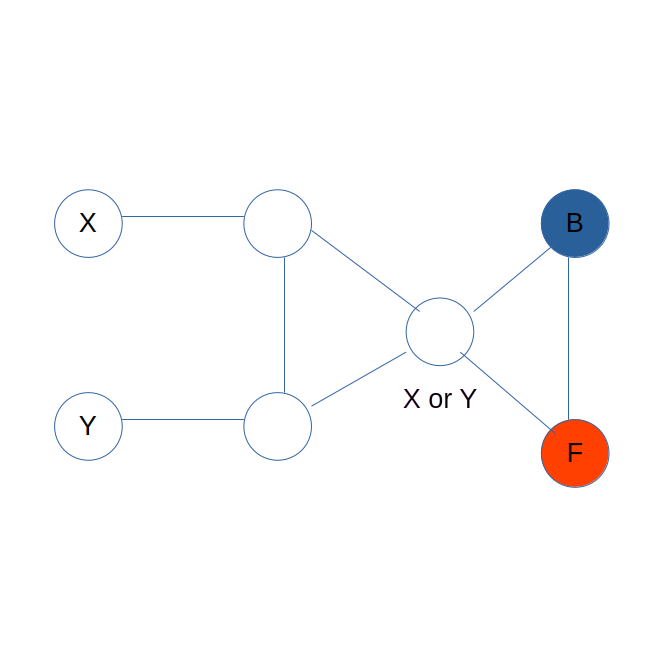
\includegraphics[width=0.5\textwidth]{or-gadget.png}
	\caption{A simple OR gadget}
\end{figure}

In the above graph, we color $x$ and $y$ accordingly and then the graph only has a valid coloring if $x \lor y$ is true.

This gadget can be easily extended to 3 variables so it can only be 3 colored if one of the variables is true. We can use this gadget to represent a clause. We use this gadget by connecting the node $x_i$ to the input node of the gadget if that node represents a variable in the corresponding clause.


To prove this reduction, we have to show that $\phi$ is satisfiable iff $G$ is 3 colored.

If $\phi$ is satisfiable, then each clause must be true. This means that each corresponding gadget must have a valid 3 coloring. If all the gadgets are 3 colored, then the graph is 3 colored.

If a graph $G$ is 3 colored, then if a node is colored $T$ iff its corresponding variable is true. If we take some clause $C_j = (a \lor b \lor c)$ then one of those variables has to be True. Otherwise the output of the gadget is false. This means that the clause is false. This means that $\phi$ is unsatisfiable. Thus it has to be satisfiable if $G$ is 3 colored.

We must also prove that this mapping is polynomial. For each clause in the formula, we have to construct a gadget that is a constant size. We have to do this for each clause in the formula. This means that the size of the graph is $O(N)$ where $N$ is the number of clauses in the formula. This is polynomial time.

Since this reduction follows, $3COL$ is NP-Complete.


\end{document}